\chapter{Background}
\label{chap:background}

This chapter introduces the theoretical background for understanding the idea
behind \texttt{Crotosolve}.
Rather than giving a complete overview of the field, this text is strictly
limited to aspects critical to proving the optimizer's correctness.
I will first present an introduction to the theory of quantum information
processing using qubits, gates, and circuits.
Following this introduction, I will also give a quick introduction to the field
of machine learning.
I will show how Quantum Machine Learning applies the ideas from machine learning
to quantum processing devices.
This section will focus on state-of-the-art classical and quantum optimization
techniques in particular.
One of these optimization methods is \texttt{Rotosolve}, which I will present
with further detail.
These basic ideas are also fundamental for the \texttt{Crotosolve}, which will
be introduced in the next chapter.

\section{A brief introduction to Quantum Computing}
At its core, the operation of a quantum computer revolves around gates and
qubits.

Qubits (quantum bits) make up the data register of a quantum computer.
Just like a classical bit can be in the $0$ or $1$ state, a qubit can be in a
corresponding $\ket 0$ or $\ket 1$ state.
Besides these two basis states, however, quantum bits can be in a superposition
of these two states,

$$\ket \psi = \alpha_0 \cdot \ket 0 + \alpha_1 \cdot \ket 1\,,$$

where the probability amplitudes $\alpha_0, \alpha_1 \in \mathbb C$ can be any
complex numbers with $\left|\alpha_0\right|^2 + \left|\alpha_1\right|^2 = 1$.
The superposable character of a qubit essentially increases its expressibility
in comparison to a classical, digital bit from the discrete set
$\left\{0, 1\right\}$ to the complex, two-dimensional sphere surface
$\left\{\vec \alpha \in \mathbb C^2 \mid \left|\vec\alpha\right|^2\right\}$.
Thus, a quantum computer with a single qubit can work with continuous,
multidimensional data, while a classical computer with a single bit can only
work with a single boolean value.

Due to the laws of quantum mechanics, this multidimensional superposition state
collapses into one of its discrete basis states upon observation.
More specifically, this means that \emph{measuring} the value of a qubit cannot
reveal its probability amplitudes and instead turns the state into either
$\ket 0$ (i.e., $\alpha_0 = 1, \alpha_1 = 0$) or
$\ket 1$ (i.e., $\alpha_0 = 0, \alpha_1 = 1$)\footnote{
    Technically, it is possible to measure the state in a different basis, like
    $\ket + = \frac{\ket 0 + \ket 1}{\sqrt 2}$ and
    $\ket - = \frac{\ket 0 - \ket 1}{\sqrt 2}$.
    However, this will not be necessary for the development of
    \texttt{Crotosolve}.
}.
The probability of the qubit collapsing into either of these states is given by
the squared absolute value of its probability amplitude,

$$\mathbb P(M = \ket n) = \left| \alpha_n \right|^2,\, n \in \left\{0, 1\right\}.$$

Thus, the normalization of the probability amplitudes, 
$\sum_{n \in \left\{0, 1\right\}} \alpha_n \ket n$, is in fact a normalization
of the probability distribution over the given basis states.
While it is physically impossible to observe $\alpha_0$ and $\alpha_1$ directly,
their squared absolute values still influence the outcome of observation $M$.
If I know how to prepare the same quantum state\footnote{
    Two quantum states $\sum \alpha_n \ket n$, $\sum \beta_n \ket n$ are the
    same if all of their probability amplitudes are the same,
    i.e., $\alpha_n = \beta_n \forall n$.
} many times, I can estimate $\left|\alpha_n\right|^2$ as the relative frequency
from an empirical probability distribution of $M$.

Since only the absolute value of $\alpha_0$ and $\alpha_1$ influences the
measurement outcome, it is common to rewrite the state as follows.

\begin{equation}
    \begin{split}
        \ket \psi
            &= \alpha_0 \ket 0 + \alpha_1 \ket 1\\
            &= e^{i\gamma} \left(\cos \frac\theta2 \ket 0 + e^{i\varphi} \sin \frac\theta2 \ket 1\right)
    \end{split}
\end{equation}

\begin{figure}
    \label{fig:blochsphere}
    \centering
    \begin{blochsphere}[radius=3 cm,tilt=15,rotation=-20,opacity=0]
        \drawBallGrid[style={opacity=0.1}]{30}{30}

        \drawAxis[]{0}{0} % Z axis
        \labelLatLon{up}{90}{0};
        \labelLatLon{down}{-90}{90};
        \node[above] at (up) {{$\left|0\right>$ }};
        \node[below] at (down) {{$\left|1\right>$}};

        \drawAxis[]{90}{0} % Y axis
        \labelLatLon{right}{0}{0};
        \labelLatLon{left}{0}{180};
        \node[right] at (right) {{$\left|R\right>$ }};
        \node[left] at (left) {{$\left|L\right>$}};

        \drawAxis[]{90}{90} % X axis
        \labelLatLon{front}{0}{90};
        \labelLatLon{back}{0}{-90};
        \node[below] at (front) {{$\left|+\right>$ }};
        \node[above] at (back) {{$\left|-\right>$}};
    \end{blochsphere}
    \caption{The Bloch sphere can represent the state of a single qubit,
        ignoring its global phase.}
\end{figure}

In this representation, $e^{i\gamma}$ has no effect on the outcome of
measurement $M$.
The remaining two variables $\theta$ and $\varphi$ can be interpreted as
coordinates on the so-called Bloch sphere, which is shown in figure
\ref{fig:blochsphere}.

\subsection{Multi-qubit-systems}
The separated state of several qubits can be combined into a multi-qubit state
through the outer product.
With two qubits, this results in

\begin{equation}
    \label{eq:separate-state}
    \begin{split}
        &\left(\alpha_0 \ket 0 + \alpha_1 \ket 1\right) \otimes \left(\beta_0 \ket 0 + \beta_1 \ket 1\right) \\
        = &\alpha_0\beta_0 \ket 0 \otimes \ket 0 + \alpha_0\beta_1 \ket 0 \otimes \ket 1 + \alpha_1\beta_0 \ket 1 \otimes \ket 0 + \alpha_1\beta_1 \ket 1 \otimes \ket 1 \\
        = &\underbrace{\alpha_0\beta_0}_{=: \gamma_{00}} \ket{00} + \underbrace{\alpha_0\beta_1}_{=: \gamma_{01}} \ket{01} + \underbrace{\alpha_1\beta_0}_{=: \gamma_{10}} \ket{10} + \underbrace{\alpha_1\beta_1}_{=: \gamma_{11}} \ket{11}.
    \end{split}
\end{equation}

with $\sum_{n \in \left\{00, 01, 10, 11\right\}} \left|\gamma_n\right|^2 = 1$.
I will use natural numbers instead of bitstrings to simplify the notation in
the following.
For example, equation \ref{eq:separate-state} can be compactly rewritten to the
following.

\begin{equation}
    \label{eq:separate-state-natural-numbers}
    \begin{gathered}
            \gamma_{00} \ket{00} + \gamma_{01} \ket{01} + \gamma_{10} \ket{10} + \gamma_{11} \ket{11}\\
        =   \gamma_0 \ket 0 + \gamma_1 \ket 1 + \gamma_2 \ket 2 + \gamma_3 \ket 3\\
        =   \sum_{j=0}^3 \gamma_j \ket j
    \end{gathered}
\end{equation}

Similarly to this two-qubit example, a system with $n$ separate qubit states
$\ket{psi_i}, 1 \leq i \leq n$ can be described with a product state.
In this system, the probability amplitudes
$\gamma_0, \dots, \gamma_{2^n -1} \in \mathbb C$ of the standard basis states
$\ket 0, \dots, \ket{2^n -1}$ are again given by the multiplication and form a
probability distribution through their squared absolute values.

\begin{equation}
    \label{eq:separate-state-n}
    \ket\psi = \bigotimes_{i=1}^n \ket{\psi_i} = \sum_{j=0^n}^{1^n} \gamma_j \ket j
        \quad\text{with}\quad \sum_{j=0}^{2^n -1} \left|\gamma_j\right|^2 = 1
\end{equation}

\subsection{Gates and circuits}

Unlike with classical bits and gates, it is physically impossible for a quantum
computer to create copies of a qubit.
While classical computers typically read (copy), transform (think add) and write
data from and to registers, quantum computers have to do all operations
in-place.

Quantum states can be changed by applying operators to them.
Since the state of an $n$-qubit-system can be described through its probability
amplitudes $\gamma_i$, we can represent this state with a $2^n$-dimensional
complex vector.
If we identify $\ket 0 \equiv \begin{pmatrix}1 & 0\end{pmatrix}^\top$ and
$\ket 1 \equiv \begin{pmatrix}0 & 1\end{pmatrix}^\top$,
equation \ref{eq:separate-state-n} leaves us with

\begin{equation}
    \ket\psi \equiv \begin{pmatrix} \gamma_{0^n} \\ \vdots \\ \gamma_{1^n}\end{pmatrix}
\end{equation}

implicitly.

Universal quantum computers allow us to apply operations to these states that
are described by unitary matrices\footnote{
    A matrix $A \in \mathbb{C}^{N \times N}$ is called unitary iff its conjugate
    transpose is its inverse, i.e. $\overline{A^\top} = A^{-1}$.
}.
% COMMONLY USED EXAMPLE GATES, PARAMETERIZABLE (CONTROLLED) ROTATIONAL PAULI
%  GATES IN PARTICULAR
% UNIVERSAL GATE SETS
% TODO: MEASUREMENTS

In Quantum Computing, every manipulation of the quantum state can be described
by a so-called gate.
A gate is a unitary transformation of the quantum state.
Gates can act on one or multiple qubits and we can compose bigger gates by
computing the outer product of gates.

We can visualize the application of gates to a system of qubits through
quantum circuits.
In these circuits, each qubit is displayed as a horizontal line and gates are
displayed as boxes that overlay the lines of the qubits they are applied to.
Measurements are indicated by a box with a meter inside.

Take for example the Hadamard gate $H$,

\begin{equation}
    H = \frac{1}{\sqrt 2}\begin{pmatrix}1 & 1 \\1 & -1\end{pmatrix}\,.    
\end{equation}

Applying the Hadamard gate to a single qubit will transform the
$\ket 0$ state into $\frac{1}{\sqrt 2}\ket 0 + \frac{1}{\sqrt 2}\ket 1$ and
$\ket 1$ into $\frac{1}{\sqrt 2}\ket 0 - \frac{1}{\sqrt 2}\ket 1$, which are
both equal superpositions of the original states.

\begin{figure}[h]
    \label{fig:H-circuit}
    \centering
    \begin{quantikz}
        \lstick{\ket{0}}    & \gate{H}  & \meter\qw
    \end{quantikz}
    \caption{
        In this single-qubit quantum circuit, a Hadamard gate is applied to the
        qubit before it is measured.
        This circuit will probablistically output $\ket 0$ just as often as
        $\ket 1$.
    }
\end{figure}

All single-qubit gates $U \in \mathbb{C}^{2 \times 2}$ can be represented by
products of \emph{pauli rotation gates} $RX(\theta), RY(\theta)$ and
$RZ(\theta)$,

\begin{equation}
    \label{eq:rotational-pauli-gates}
    RP\left(\theta\right) = \cos\left(\frac\theta2\right) \cdot I_2 - i \cdot \sin\left(\frac\theta2\right) \cdot P,\quad
    P \in \left\{X, Y, Z\right\}
\end{equation}

These gates are called \emph{parameterized gates} since they can be adjusted by a
continuous parameter $\varphi \in \left[0, 2\pi\right]$.
The Hadamard gate, for example, can be written as
$H = RX(\pi) \cdot RY(0.5\pi)$.

Single-qubit operations can be simulated trivially by computing the product of
the gate matrices and the state vector.

The problem gets more interesting with two-qubit gates.
For example, the controlled $X$ gate (also known as $CNOT$) works on a system
of two qubits and maps the basis states as follows:

\begin{gather}
    \label{eq:cx-zbasis}
    CX = \begin{pmatrix}
        1&0&0&0\\
        0&1&0&0\\
        0&0&0&1\\
        0&0&1&0
    \end{pmatrix}\\
    CX \ket{00} = \ket{00}\\
    CX \ket{01} = \ket{01}\\
    CX \ket{10} = \ket{11}\\
    CX \ket{11} = \ket{10}
\end{gather}

When applying the $CX$ gate to states from the computational basis, the second
bit is flipped ($X$ is applied) iff the first bit is $\ket 1$.
States other than those from the computational basis might, however, not follow
this simple principle.
The $\ket{++}$ state, for example, is transformed into the
$\ket{-+} = CX \ket{++}$ state, changing the control qubit but not the target
qubit.

\section{Quantum Machine Learning}
Parameterized quantum circuits realize a mapping from an input state to an
output state.
This mapping can be considered an algorithm that is determined by parameters of
the PQC.
If the PQC is expressible enough, tweaking the parameters can lead to an
arbitrary function.

This setup is very similar to the one used in classical machine learning.
In supervised learning scenarios, the labeled training data is typically fed
into a black-box model to generate an output that is supposed to be similar to
the data's label.
The black-box model is an algorithm -- for example, a neural network -- expected
to be capable of expressing the mapping from the input data to its labels that
can be tweaked using a potentially large set of parameters.
Comparing the output of the model and the expected output yields a loss value,
quantitatively representing the error of the model.
Using this loss value, an optimizer's task then is to change the black-box
model's parameters so that the loss in the next iteration will be smaller.

\begin{figure}[h]
    \label{fig:ml-training-loop}
    \centering
    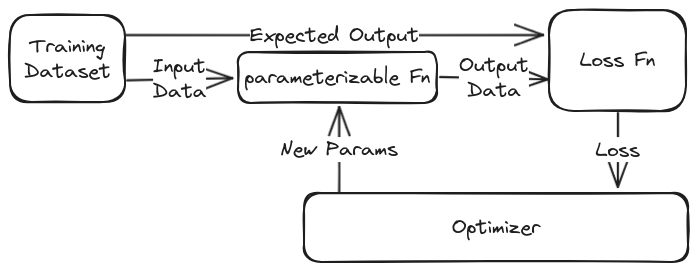
\includegraphics[width=0.8\textwidth]{ml-training-loop}
    \caption{A typical machine learning optimization loop}
\end{figure}

Quantum machine learning makes use of this exact same setup by using a
parameterized quantum circuit as the parameterizable black-box model in the
optimization loop.

\subsection{Optimization techniques}

\section{Outline}
Background: Quantum computing and QML with PQCs
\begin{itemize}
    \item
        Briefly explain the operation of a quantum computer
        \cite{nielsen_quantum_2007}.
        This section should mention qubits, gates, universal gate sets,
        measurements and their mathematical representation.
        Make sure to mention parameterizable gates like rotational pauli (RP)
        gates and controlled rotational pauli (CRP) gates.
    \item
        Explain the setup for quantum machine learning with parameterized
        quantum circuits (PQCs) \cite{mitarai_quantum_2018}.
        Mention the analogy of quantum machine learning with PQCs with
        classical machine learning setups \cite{bishop_pattern_2006}.
        This section should include a few examples and cite demonstrations
        as well as evaluations of the idea.
    \item
        Go into detail on the different optimization techniques used for
        this approach.
        This section should mention state-of-the-art optimizers such as
        Adam \cite{kingma_adam_2017}, Gradient Descent and
        % TODO: cite gradient descent?
        (Quantum) Natural Gradient \cite{stokes_quantum_2020}.
        % TODO: SPSA instead of QNG?
        Also explain the parameter shift rule
        \cite{mitarai_quantum_2018,schuld_evaluating_2019} as we are trying
        to replace it.
        % TODO: re-formulate
        % TODO: maybe explain fourier sums too
\end{itemize}
